
\chapter{Computational Methods} % Main chapter title

\label{Chapter3} % Change X to a consecutive number; for referencing this chapter elsewhere, use \ref{ChapterX}
%\doublespacing

\section{Molecular Dynamics}

\subsection{Background and Formulation}
Molecular Dynamics (MD) uses molecular configurations (Cartesian coordinates and momentum) to extract structural, thermodynamic, and dynamic information of a system. This information is extracted from the time evolution of the system, which is obtained  through the numerical integration of the Newton's equations of motion \cite{tuckerman}:

\begin{equation}
\frac{d \vec{p}_{i}}{dt} = - \frac{\partial U (\vec{r}_{N})}{\partial \vec{r}_{i}},
\end{equation}
where $p_{i}$ is the momentum and $r_{N}$ are the coordinates of all the atoms $(x_{1},y_{1},z_{1},..., x_{N},\\ y_{N},z_{N})$. Alternatively, we can write the equation relative to the velocity ($v_{i}$):
\begin{equation}
m_{i} \frac{\vec{v}_{i}}{dt} = - \frac{\partial U (\vec{r}_{N})}{\partial \vec{r}_{i}}.
\end{equation}

In order to develop equations for any coordinate system, for instance $q^{N}=(r_{1},\theta _{1},\phi _{1})$, the Hamiltonian formulation, a more general formulation of classical mechanics,  is used to develop the equations of motion:
\begin{equation}
\mathcal{H} (q^{N},p^{N}) = K(p^{N}) + U(q^{N}) .
\end{equation}

In the equation above, $K$ is the kinetic energy and $U$ is the potential energy. The equations of motion are then rewritten using the Hamiltonian:

\begin{equation}
\frac{d \vec{p}_{i}}{dt} = - \frac{\partial \mathcal{H}}{\partial \vec{q}_{i}},
\end{equation}

\begin{equation}
\frac{d \vec{q}_{i}}{dt} =  \frac{\partial \mathcal{H}}{\partial \vec{q}_{i}}.
\end{equation}

In the dynamics described by the equations above, the Hamiltonian is preserved. The coordinate and momentum axes for each atom in a 6N dimensional space is defined as the phase space. The trajectory through the phase space is then the time evolution of a system in a molecular dynamics simulation. This evolution of the simulation may be used to calculate the thermodynamic properties if the system is ergodic, that is, a trajectory in this system will explore with the same probability all regions of the phase space of microstates (points in phase space) with the same energy \cite{shell2015}. 

\subsection{Statistical Ensembles}

In order to calculate thermodynamic properties, we need to define the control variables of a system. For an isolated system at equilibrium, the control variables are the number of particles (N), volume (V), and total energy (E). The set of configurations under the control variables is then called statistical ensemble. In the example cited above, it is specifically named the microcanonical ensemble. Following the ergodic hypothesis, the system at these conditions will spend the same amount of time in each of the microstates  with the fixed Hamiltonian.  The number of accessible microstates is defined by the partition function or the density of states, and  is given by the following equation  for the microcanonical ensemble: 

\begin{equation}
\begin{aligned}
\Omega (N,V,E) = \frac{\epsilon_{0}}{h^{3N}N!} \int dp^{N} dr^{N} \delta [\mathcal{H}(p^{N},r^{N}) -E].
\end{aligned}
\end{equation}

Here, $\epsilon _{0}$ is the energy unit, $h$ is the Planck constant, and $\delta$ is the Dirac delta function. As mentioned above, the system will spend the same amount of time at each of the microstates, i. e. each of these microstates have equal probabilities ($\varrho$) of being visited. Such probability is:

\begin{equation}
\begin{aligned}
\varrho (p^{N},r^{N}) = \frac{[\mathcal{H}(p^{N},r^{N}) -E]}{ \Omega (N,V,E)} .
\end{aligned}
\end{equation}

The macroscopic properties from molecular dynamics are then obtained from the relation of the microcanonical partition function to the entropy ($S$). Known as the Boltzmann equation. It is:

\begin{equation}
\begin{aligned}
S = \kappa_{b} ln [\Omega (N,V,E)], 
\end{aligned}
\end{equation}
where $\kappa_{b}$ is the Boltzmann constant. With these equations, we can derive other relations to macroscopic properties with the fundamental thermodynamic equations:

\begin{equation}
\begin{aligned}
dS = \frac{1}{T} dE + \frac{P}{T} dV + \frac{\mu}{T} dN,
\end{aligned}
\end{equation}

\begin{equation}
\begin{aligned}
dE = T dS + P dV + \mu dN .
\end{aligned}
\end{equation}

As said above, the microcanonical ensemble  has  N, V, and E as its control variables. Other ensembles can also be defined according to the macroscopic properties held constant.  In the canonical ensemble,  N, V, and the temperature (T) are held constant and  N, pressure (P), and T are held constant in the isothermal-isobaric ensemble. Other ensembles are the isoenthalpic-isobaric (constant number of particles, pressure, and enthalpy) and the grand canonical (constant chemical potential, volume, and temperature) ones. A variety of physical properties is measured at the conditions of the isothermal-isobaric ensemble such as enthalpies, entropies, redox potential, equilibrium constants, and free energies, what makes this ensemble one of the most important \cite{tuckerman}. This is also the ensemble in which solvation free energy simulations are carried out at this work, hence we are going to briefly talk about it. This ensemble is obtained from a Legendre transformation on the canonical ensemble. The Helmholtz free energy $A(N,V,T)$ becomes the Gibbs free energy $G(N,P,T)$ by transforming the volume into the external pressure:
\begin{equation}
G(N,P,T) = A(N,V,T) + PV,
\end{equation}
where $V = V(P)$. The Gibbs free energy is related to its partition function $\Delta (N,P,T)$ by:

\begin{equation}
\label{eq:fisobari}
\begin{aligned}
G(N,P,T) = -\kappa_{b}T ln \Delta (N,P,T),
\end{aligned}
\end{equation}
where $\Delta (N,P,T)$ is given by: 

\begin{equation}
\begin{aligned}
\Delta (N,P,T) = \frac{1}{V_{0}} \int_{0}^{\infty} dV \int d p^{N} d r^{N} \exp \left[ -\beta \left( \mathcal{H} (r^{N},p{N}) + PV(r^{N}) \right) \right] .
\end{aligned}
\end{equation}

In the equation above, $Q (N,V,T)$ is the partition function of the canonical ensemble:

\begin{equation}
\begin{aligned}
Q(N,V,T) = \int d^{N}p d^{N}r \exp \left[ -\beta \mathcal{H} (r^{N},p{N}) .
\right]
\end{aligned}
\end{equation}

From these relations and a differential change in G, we can obtain the chemical potential ($\mu$), volume and entropy relations for isothermal-isobaric ensemble:

\begin{equation}
\mu = \left (\frac{\partial G}{\partial N} \right)_{P,T} = - \kappa_{b} T \left(\frac{\partial ln \Delta (N,P,T)}{\partial N} \right)_{N,T},
\end{equation}  
\begin{equation}
\langle V \rangle= \left (\frac{\partial G}{\partial P} \right)_{N,T}= \kappa_{b} T \left (\frac{\partial ln \Delta (N,P,T)}{\partial N} \right)_{N,P},
\end{equation}
\begin{equation}
S = \left (\frac{\partial G}{\partial T} \right)_{N,P}= \kappa_{b}  \left[ln Q(N,V,T)+ T \left (\frac{\partial ln Q (N,V,T)}{\partial T} \right)_{V,N}\right] .
\end{equation}

\subsection{Thermostats and Barostats}

The isothermal-isobaric and canonical ensembles have external conditions being applied to it (temperature and pressure). For temperature control, the method employed mimics the effect of a thermal reservoir through the use of a thermostat. The thermostats need to be capable of capturing the correct energy fluctuations in the system since the kinetic energy will fluctuate when using a heat bath to control the temperature in a canonical ensemble of a finite system \cite{frenkel}.  

Among the available thermostat are the Berendsen \cite{doi:10.1063/1.448118}, the Andersen \cite{1980JChPh722384A}, and the Nos\'{e} \cite{1984JChPh81511N} thermostats, but, here, we are going to discuss the most widely used thermostat: the Nosé-Hoover \cite{PhysRevA.31.1695}. This thermostat is based on the formulation of Nosé \cite{1984JChPh81511N}, who used a Lagrangian that contains additional and artificial coordinates and velocities \cite{frenkel}. In this method, the Hamiltonian in a canonical ensemble is constructed as:

\begin{equation}
\mathcal{H}_{Nos\acute{e}} =  K(p^{N}) + U(q^{N})  + \frac{\xi ^{2} \mathcal{Q}}{2} + 3N\kappa_{b}T ln s ,
\end{equation}
where $\xi$ is a friction coefficient related to the conjugate momentum of the thermal reservoir to which the system is coupled, $s$ is the position of the thermal reservoir, and $\mathcal{Q}$ is the effective mass associated with s. The velocity update is then done with the friction term added to the equations of motion \cite{shell2015}:

\begin{equation}
\frac{dr_{i}}{dt} = \frac{p_i}{m_i},
\end{equation}

\begin{equation}
\frac{dp_{i}}{dt} = -  \frac{\partial U (r^{N})}{\partial r_{i}} - \xi p_{i},
\end{equation}

\begin{equation}
\frac{\xi}{dt} = \frac{\sum p_{i}^{2}/m_{i} - 3N\kappa_{b}T}{\mathcal{Q}} ,
\end{equation}

\begin{equation}
\frac{1}{s}\frac{ds}{dt} =\frac{d \ln s}{dt} = \xi.
\end{equation}

This approach proposed by the Nos\'{e}-Hoover thermostat only generates a correct canonical distribution for molecular systems in which there are no external forces ($F_{i}$) and the center of mass is fixed or if there is only one conserved quantity \cite{frenkel}. To diminish these restrictions of the Nosé-Hoover thermostat, the Nosé-Hoover chains of thermostats method was developed by \citeonline{doi:10.1063/1.463940}. This is the one chosen to control the temperature in our simulations. It proposes the use of another thermal reservoir or a whole chain of thermal reservoirs in order to enhance temperature equilibration \cite{shell2015}. Here, we are going to present its equations of motion since this was the method used in this dissertation. The equations of motion of a system of N particles coupled with M Nos\'{e}-Hoover chains is given by

\begin{equation}
\frac{dr_{i}}{dt} = \frac{p_i}{m_i},
\end{equation}

\begin{equation}
\frac{dp_{i}}{dt} = F_i  - \frac{p_{\xi _{1}}}{\mathcal{Q} _1} p_{i},
\end{equation}

\begin{equation}
\frac{\xi _{k}}{dt} = \frac{p_{\xi _k}}{\mathcal{Q} _{k}} \quad k = 1,...,M ,
\end{equation}

\begin{equation}
\frac{p_{\xi _1}}{dt} = {\sum p_{i}^{2}/m_{i} - 3N\kappa_{b}T} -  \frac{p_{\xi _{2}}}{\mathcal{Q} _2}p_{\xi _{1}},
\end{equation}

\begin{equation}
\frac{p_{\xi _k}}{dt} = \frac{p_{\xi _{k -1}}^{2}}{\mathcal{Q} _{k-1}} - \kappa_{b}T - \frac{p_{\xi _{k+1}}}{\mathcal{Q} _{k+1}}p_{\xi _{k}},
\end{equation}

\begin{equation}
\frac{p_{\xi _M}}{dt} = \frac{ p_{\xi _{M-1}}^{2}}{\mathcal{Q} _{M-1}} - \kappa_{b}T .
\end{equation}

The conserved energy for the Nos\'{e} Hoover chains is then equal to

\begin{equation}
\mathcal{H}_{Nos\acute{e} \, Chains} =  K(p^{N}) + U(q^{N})  + \sum_{k=1}^{M }\frac{p^{2}_{\xi _{k}}}{2\mathcal{Q} _{k}} + 3N\kappa_{b}T \xi _{1} + \sum_{k=2}^{M} \kappa_{b}T \xi _{k}.
\end{equation}

The pressure is controlled with a barostat. It maintains the pressure constant during the simulation by adjusting the simulation volume. Among the available  barostats methodologies are the Berendsen \cite{doi:10.1063/1.448118}, in which the pressure is coupled to a pressure bath, and the volume is periodically rescaled, and the Anderson barostat \cite{1980JChPh722384A}, which serves as a basis for other barostating methods such as the ones developed by Hoover \cite{PhysRevA.31.1695}, Martina-Tobias-Klein \cite{doi:10.1063/1.467468} and Parrinello-Rahman \cite{doi:10.1063/1.328693}. The Andersen's idea was to couple the system to a fictional pressure bath and incorporate the volume into the phase space as an additional degree of freedom \cite{tuckerman}. Here, we are going to present the approach developed by \citeonline{doi:10.1063/1.467468} since this was the one used to control the pressure in our simulations. The equations of motion for a chain of barostats of length M are given by  

\begin{equation}
\frac{dr_{i}}{dt} = \frac{p_i}{m_i} + \frac{p_{\epsilon}}{\mathcal{W}} r_i,
\end{equation}

\begin{equation}
\frac{dp_{i}}{dt} = F_i  - \left(1 + \frac{d}{dN}\right) \frac{p_{\epsilon}}{\mathcal{W}} p_{i} - \frac{p_{\epsilon _{1}}}{\mathcal{Q} _1} p_{i},
\end{equation}

\begin{equation}
\frac{dV}{dt} = \frac{d V p_{\epsilon}}{\mathcal{W} }
\end{equation}

\begin{equation}
\frac{dp_{\epsilon}}{dt} = dV (    P_{int} -P_{ext}) + \frac{1}{N} \sum_{i=1}^{N} \frac{p_{i}^{2}}{m_i} - \frac{p_{\xi _{1}}}{{\mathcal{Q} _1}}p_{\epsilon},
\end{equation}

\begin{equation}
\frac{\xi _{k}}{dt} = \frac{p_{\xi _k}}{\mathcal{Q} _{k}} \quad k = 1,...,M ,
\end{equation}

\begin{equation}
\frac{p_{\xi _1}}{dt} = \sum \frac{p_{i}^{2}}{m_{i}} - \frac{p_{\epsilon}^{2}}{\mathcal{W}} -  (dN +1)\kappa_{b}T -\frac{p_{\xi _{2}}}{\mathcal{Q} _2}p_{\xi _{1}},
\end{equation}

\begin{equation}
\frac{p_{\xi _k}}{dt} = \frac{p_{\xi _{k -1}}^{2}}{\mathcal{Q} _{k-1}} - \kappa_{b}T - \frac{p_{\xi _{k+1}}}{\mathcal{Q} _{k+1}}p_{\xi _{k}} \quad k = 2,...,M-1 ,
\end{equation}

\begin{equation}
\frac{p_{\xi _M}}{dt} = \frac{ p_{\xi _{M-1}}^{2}}{\mathcal{Q} _{M-1}} - \kappa_{b}T .
\end{equation}

In the equations above, $\epsilon$ is equal to

\begin{equation}
\epsilon = \ln \left[\frac{V}{V(0)}\right],
\end{equation}
where $V$ is the volume of the system and $V(0)$ is the volume at $t=0$. The mass parameter ($\mathcal{W}$) associated to $\epsilon$, the momentum ($p_{\epsilon}$) conjugate to $\epsilon$, the external pressure ($P_{ext}$), and the internal pressure ($P_{int}$) are also featured in the equations of motion. $P_{ext}$ is imposed as we do with the temperature in the thermostat and $P_{int}$ is calculated during the simulation with the following equation \cite{tuckerman}:

\begin{equation}
P_{int} = \frac{1}{dV} \left[\sum_{i=1}^{N} \left(\frac{p_{i}^2}{m_i} + r_{i}\cdot F_i \right) - dV \frac{\partial U}{\partial V}\right].
\end{equation}


Finally, the conserved energy for the chain of barostats proposed by \citeonline{doi:10.1063/1.467468} is equal to

\begin{equation}
\mathcal{H}_{N,P_{ext},T} =  K(p^{N}) + U(q^{N})  + \frac{p_{\epsilon}^2}{\mathcal{W}}+\sum_{k=1}^{M }\frac{p^{2}_{\xi _{k}}}{\mathcal{Q} _{k}} + (dN+1)\kappa_{b}T \xi _{1}  + \kappa_{b}T\sum_{k=1}^{M}  \xi _{k} + P_{ext}V.
\end{equation}

All the equations of motion above are then numerically integrated  using the methodologies described in the next section.

\subsection{Integration of the equations of motion}

With the formalism defined for the equations of motions and the statistical ensemble, we can now derive discrete-time numerical approximations for them.  The basic idea is to solve the trajectory of atoms as a function of time [$r^{N}(t)$] by updating the positions at discrete time intervals or time steps. To do that, the classical time evolution approach is used to preserve the Hamiltonian of the system in the numerical integration methods. In this approach, we consider the time evolution of an arbitrary function $a(x_{t})$ along a trajectory $x_{t}$ \cite{tuckerman}. Doing the time derivative of $a(x_{t})$:

\begin{equation}
\frac{da}{dt} = \sum_{\alpha=1}^{3N} \left [  \dfrac{\partial \mathcal{H}}{\partial p_{\alpha}}\dfrac{\partial a}{\partial q_{\alpha}}  -  \dfrac{\partial \mathcal{H}}{\partial q_{\alpha}} \dfrac{\partial a}{\partial p_{\alpha}} \right].
\label{eqn:operador}
\end{equation}

In the equation above, we can represent the time evolution of $a(x_{t})$ with  the Poisson bracket:

\begin{equation}
\frac{da}{dt} = \{a,\mathcal{H}\}.
\end{equation}

The Poisson bracket is equal to applying the Liouville operator ($i\mathcal{L}$) on the phase space. Hence,

\begin{equation}
\begin{aligned}
\frac{da}{dt} = i\mathcal{L} a .
\end{aligned}
\label{eqn:liou}
\end{equation}

Substituting Eq. \ref{eqn:liou} in Eq. \ref{eqn:operador}, we have the following equation:

\begin{equation}
\begin{aligned}
i\mathcal{L} a = \sum_{\alpha=1}^{3N} \left [  \dfrac{\partial \mathcal{H}}{\partial p_{\alpha}}\dfrac{\partial a}{\partial q_{\alpha}}  -  \dfrac{\partial \mathcal{H}}{\partial q_{\alpha}} \dfrac{\partial a}{\partial p_{\alpha}} \right].
\label{eqn:liou2}
\end{aligned}
\end{equation}

The solution of Eq. \ref{eqn:liou} for $a(x_{t})$ is given by

\begin{equation}
a(x_{t}) = \exp (i\mathcal{L}t) a(x_{0}).
\label{eqn:exactsol}
\end{equation}

Here, $\exp (i\mathcal{L}t)$ is known as the classical propagator. The effect of this operator in a function can not be evaluated. However, we can develop approximate solutions for the Hamiltonian's equations with this operator \cite{tuckerman}. Rewriting Eq. \ref{eqn:liou2} as

\begin{equation}
\begin{aligned}
i\mathcal{L}  =  i\mathcal{L}_{1} + i\mathcal{L}_{2},
\end{aligned}
\end{equation}
where
\begin{equation}
\begin{aligned}
i\mathcal{L}_{1} = \sum_{\alpha=1}^{N}  \dfrac{\partial }{\partial q_{\alpha}} \dfrac{\partial \mathcal{H}}{\partial p_{\alpha}},   \\
i\mathcal{L}_{2} = - \sum_{\alpha=1}^{N} \dfrac{\partial }{\partial p_{\alpha}} \dfrac{\partial \mathcal{H}}{\partial q_{\alpha}} .
\end{aligned}
\end{equation}

The operators $i\mathcal{L}_{1}$ and $i\mathcal{L}_{2}$ in the equations above are non-commuting operators, that is, the order in which the operator is applied is important \cite{tuckerman}. This fact implies that we can not separate the classical propagator $\exp (i\mathcal{L}t)$  into the product $\exp (i\mathcal{L}_{1}t) \exp (i\mathcal{L}_{2}t)$. Though we can not do that, we can still express the propagator in terms of these two factors by using the symmetric Trotter theorem or Strang splitting formula \cite{trotter,strang}. Applying this theorem to the classical propagator, we then obtain

\begin{equation}
\begin{aligned}
\exp (i\mathcal{L}t)  = \exp (i\mathcal{L}_{1}t + i\mathcal{L}_{2}t) = \\
\lim\limits_{P \rightarrow \infty} \left [ \exp (i\mathcal{L}_{2}t/2P) \exp (i\mathcal{L}_{1}t/P) \exp (i\mathcal{L}_{2}t/2P) \right ]^{P},
\end{aligned}
\label{eqn:trotter}
\end{equation}
where P is an integer. Defining a time step $\Delta t =t/P$ and using it in Eq. \ref{eqn:trotter}, we have

\begin{equation}
\begin{aligned}
\exp (i\mathcal{L}t)  = 
\lim\limits_{P \rightarrow \infty, \Delta t \rightarrow 0} \left [ \exp (i\mathcal{L}_{2} \Delta t/2) \exp (i\mathcal{L}_{1} \Delta t) \exp (i\mathcal{L}_{2} \Delta t/2) \right ]^{P}.
\end{aligned}
\label{eqn:trotterdt}
\end{equation}

In order to obtain an approximation for $\exp (i\mathcal{L}t)$, we do not take the limits and consider that P is a finite number \cite{tuckerman}. The resulting approximation for the classical propagator is then 

\begin{equation}
\begin{aligned}
\exp (i\mathcal{L}t)  \equiv
\left [ \exp (i\mathcal{L}_{2} \Delta t/2) \exp (i\mathcal{L}_{1} \Delta t) \exp (i\mathcal{L}_{2} \Delta t/2) \right ]^{P} + \vartheta (P \Delta t^{3}),
\end{aligned}
\end{equation}
using $P= t/\Delta t$
\begin{equation}
\begin{aligned}
\exp (i\mathcal{L} \Delta t)  \equiv
\exp (i\mathcal{L}_{2} \Delta t/2) \exp (i\mathcal{L}_{1} \Delta t) \exp (i\mathcal{L}_{2} \Delta t/2)  + \vartheta (\Delta t^{3}).
\end{aligned}
\label{eqn:trotterfin}
\end{equation}  

Now we can use Eq. \ref{eqn:trotterfin} as a numerical propagation for a single time step ($\Delta t$). Using this propagation on a single particle moving with Hamiltonian, where $i\mathcal{L}_{1} = K (p)$ and $i\mathcal{L}_{2} = U (r)$, we obtain

\begin{equation}
\begin{aligned}
\exp (i\mathcal{L} \Delta t)  \equiv
\exp \left (-\frac{\Delta t}{2} \dfrac{\partial U}{\partial r} \dfrac{\partial}{\partial p} \right) \exp \left( \Delta t \frac{p}{m}\dfrac{\partial }{\partial r} \right)\exp \left (-\frac{\Delta t}{2} \dfrac{\partial U}{\partial r} \dfrac{\partial}{\partial p} \right) ,
\end{aligned}
\label{eqn:trotterfin2}
\end{equation} 
where the derivatives of the intermolecular potential $-\dfrac{\partial U(r)}{\partial r}$ are equal to the force ($F$) acting on the particle. We now are able to replace the exact solution of Eq. \ref{eqn:exactsol} with the approximation of Eq. \ref{eqn:trotterfin2}. The approximation evolution from a initial condition $(r(t),p(t))$  is then

\begin{equation}
\begin{aligned}
\left[ \begin{array}{c} r(t+ \Delta t) \\ p(t + \Delta t) \end{array} \right] \equiv 
\exp \left (\frac{\Delta t}{2} F(r(t)) \dfrac{\partial}{\partial p} \right) 
\times \exp \left( \Delta t \frac{p(t)}{m}\dfrac{\partial }{\partial r} \right) \\
\times \exp \left (\frac{\Delta t}{2} F(r(t)) \dfrac{\partial}{\partial p} \right)
\left[ \begin{array}{c} r(t) \\ p(t) \end{array} \right] .
\end{aligned}
\end{equation}

The propagation is determined by acting each of the three operators starting from the right on $r$ and $p$. The result of applying the operator in a function $g(r)$ is the Taylor expansion $g(r+c)$. Hence,  after applying the first operator, we obtain the equation bellow \cite{tuckerman}:

\begin{equation}
\begin{aligned}
\exp \left \lbrace \frac{\Delta t}{2} F[r(t)] \dfrac{\partial}{\partial p} \right \rbrace
\left[ \begin{array}{c} r(t) \\ p(t) \end{array} \right] = 
\left[ \begin{array}{c} r(t) \\ p(t) + \frac{\Delta t}{2} F(r(t)) \end{array} \right] .
\end{aligned}
\end{equation}

Acting the second operator in the preceding equation, the result is the following:

\begin{equation}
\begin{aligned}
\exp \left[ \Delta t \frac{p(t)}{m}\dfrac{\partial }{\partial r} \right]
\left[ \begin{array}{c} r(t) \\ p(t) + \frac{\Delta t}{2} F[r(t)] \end{array} \right] = 
\left[ \begin{array}{c} r(t) + \frac{\Delta t}{m}p(t) \\ p(t) + \frac{\Delta t}{2} F[r(t) + \frac{\Delta t}{m}p(t) ] \end{array} \right] .
\end{aligned}
\end{equation}
and, finally, we find the following equations after applying the third operator :

\begin{equation}
\begin{aligned}
\exp \left \lbrace \frac{\Delta t}{2} F[r(t)] \dfrac{\partial}{\partial p} \right \rbrace
\left[ \begin{array}{c} r(t) + \frac{\Delta t}{m}p(t) \\ p(t) + \frac{\Delta t}{2} F[r(t) + \frac{\Delta t}{m}p(t) ] \end{array} \right]= \\ 
\left[ \begin{array}{c} r(t) + \frac{\Delta t}{m} \lbrace p(t)+\frac{\Delta t}{2} F[r(t)]\rbrace \\ p(t) + \frac{\Delta t}{2} F[r(t)] + \frac{\Delta t}{2} F\{r(t)+ \frac{\Delta t}{m} [p + \frac{\Delta t}{2}F(r(t))]\}\end{array} \right] .
\end{aligned}
\end{equation}

Using the equations above and substituting $p/m$ for $v$, the final position $r(t+\Delta t)$ can be written as

\begin{equation}
r(t+ \Delta t) = r(t) +v(t) \Delta t + \frac{F(t)}{2m} \Delta t^{2}.
\label{eqn:verlet}
\end{equation}

Eq.  \ref{eqn:verlet} is the position update part of the velocity-Verlet algorithm \cite{verlet}. In this method, the positions are updated by a time step of $\Delta t$ by using the positions at the previous time steps and forces. These recalculations of forces at each time step are the most computationally expensive part of the simulation since we have to take the derivative of the potential energy at each time step. The equation to update the velocity can also be derived from the equations above. It is given by

\begin{equation}
v(t+ \Delta t) = v(t) +\frac{F(t+ \Delta t) +F(t)}{2m} \Delta t .
\end{equation}

Instead of using a time step of $\Delta t$, the velocities can be updated at $\Delta t /2$. This is the strategy proposed by the leap frog algorithm:

\begin{equation}
v(t+ \Delta t /2) = v(t- \Delta t /2) +\frac{F(t+ \Delta t) +F(t)}{m} \Delta t ,
\end{equation}

\begin{equation}
r(t+ \Delta t) = r(t) +v(t+ \Delta t /2) \Delta t .
\end{equation}

Although using different time steps or formulations, both of the methods described here generate the same trajectory for a given initial configuration.

\subsection{Initial Configuration and Periodic Boundary Condition} \label{icbc}

The equations from the preceding section require an overlap-free initial configuration with positions and velocities for all atoms in the system. The initial velocities follow a temperature-dependent Maxwell-Boltzmann distribution, which is

\begin{equation}
\varrho (v_{x,i}) = \left (\frac{m_{i}}{2 \pi \kappa_{b} T} \right )^{\frac{1}{2}} \exp \left (-\frac{m_{i}v_{x,i}^2}{2 \pi \kappa_{b} T} \right) .
\end{equation}

Random velocities are then found with the equation above for each of the 3N components of the velocity, and the initial positions can be obtained by several approaches. The initial configuration can be taken from an x-ray or a nuclear magnetic resonance (NMR) spectroscopy, the atoms can be placed randomly in the simulation volume, or the atoms can be placed in idealized or approximate geometries. The generally used method to acquire the configurations places the molecules on a cubic lattice \cite{shell2015}.  Among the available software to optimize this placement, there is the Packmol software \cite{packmol}. It treats the initial configuration problem as a packing optimization problem. The molecules are packed in such way that atoms from different molecules keep a safe pairwise distance and, due to the optimization function and gradient evaluations, this strategy enables the packing of millions of atoms in reasonable time \cite{packmol}.   

Independently of the technique or software used, certain restrictions should be applied in the initial configurations to carry out molecular simulations. As an example, the cubic lattice has a finite size, but a finite box would result in simulations dominated by surface effects. To avoid that and be able to simulate bulk phase, we can create a box periodically repeated in all directions by applying the so-called Periodic Boundary Conditions (PBC) \cite{frenkel}. The periodic box has a primitive cell, which contains the N particles, replicated in a periodic lattice of infinite cells as represented in Figure \ref{fig:pbc}. 

\begin{figure}[h]
	\centering
	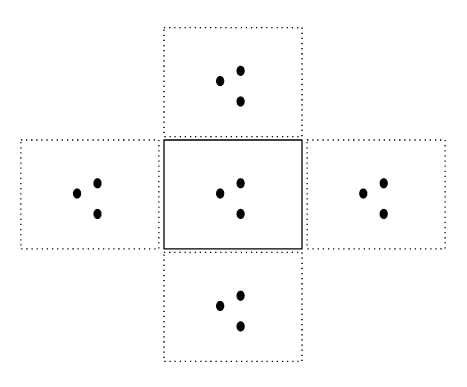
\includegraphics[width=0.7\textwidth]{Figures/pbc}
	\caption{Representation of the periodic boundary condition.}
	\label{fig:pbc}
\end{figure}

The application of the PBC results in particles interacting not only with each other but also with their images. This fact significantly increases the number of interacting pairs and, consequently, the computational time. To overcome that, we need to choose a limited range potential using the minimum image convention criterion. This criterion only allows a particle to interact with the nearest particle or image.  This is technically done during the simulations by neglecting the interactions between two particles at or beyond a maximum length, which is given the name of cutoff radius ($R_{c}$). This cutoff should be equal to or less than half of the box length. This process of examining each pair separation can also be expensive depending on the number of distinct pairs. That is the reason molecular dynamics algorithms use pair listings. This method defines a 'skin' around the cutoff radius with a radius $R_{List}$, as represented in Figure \ref{fig:pairlist}. The pair list is initially built of all the neighbor particles within a distance $R_{List}$ of each particle. Over the course of the simulation, only pairs in the pair list interact. We then will have a list of all particles j with which a particle i interacts as an example. The pair list must then be updated from time to time during the simulation since particles typically diffuse \cite{tuckerman}.    

\begin{figure}[h]
	\centering
	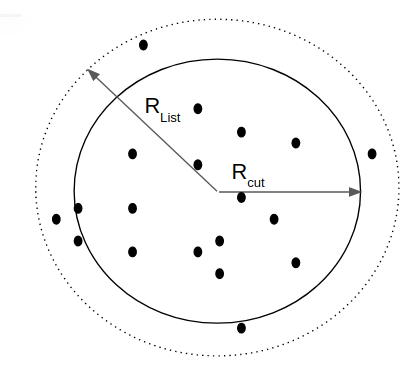
\includegraphics[width=0.5\textwidth]{Figures/pairlist}
	\caption{Representation of the cutoff radius and the pair list radius. Adapted from \citeonline{tuckerman}.}
	\label{fig:pairlist}
\end{figure}

\subsection{Force Fields }
As said previously, we need to calculate the derivative of the potential energy function in relation to the coordinates in order to update the positions during a simulation. Therefore, we need a model for this potential energy functions. These models are called force fields. They can describe structural characteristics such as van der Waals interactions, bond lengths, bond angles, and torsion in a molecular simulation. The description is done by approximating the potential energy function [$U(r^N)$], which has contributions due to intermolecular and intramolecular interactions. The intramolecular interactions include bond stretching, angle bending, and bond torsion. An illustration of these interactions can be seen in Figure \ref{fig:intraint}. 

\begin{figure}[H]
	\centering
	[a]{{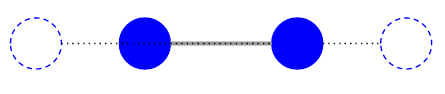
\includegraphics[width=.3\textwidth]{Figures/bondstrech} }}%
	\qquad
	[b]{{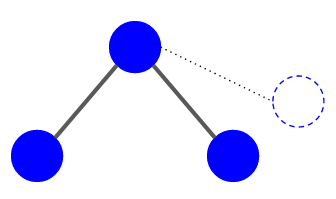
\includegraphics[width=.3\textwidth]{Figures/anglebend} }}%
	\qquad
	[c]{{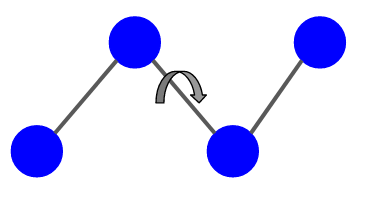
\includegraphics[width=.3\textwidth]{Figures/torsion} }}%    
	\caption{Representation of bond stretching [a], angle bending [b], and bond torsion [c].}%
	\label{fig:intraint}%
\end{figure}


At this dissertation, we are going to present the equations which are most used to represent these interactions. The contribution to the bond stretching (bs ) is usually given by the harmonic approximation around the energy minimum:

\begin{equation}
u_{bs}(d) = k_{bs} (d - d_{0})^2 .
\end{equation}

Here, $d$ is the bond length, $d_{0}$ is the equilibrium bond length, and $k_{bs}$ is a bond stretching constant. The angle bending (ab) contribution corresponds to deviations from the preferred geometry and is often given by:

\begin{equation}
u_{ab}(\theta) = k_{ab} (\theta - \theta _{0})^2,
\end{equation}
where $k_{ab}$ and $\theta _{0}$ are constants defined by the force field and $\theta$ is the bond angle between three atoms.  The bond torsion (bt) interactions correspond to the energies of rotations around bonds, and it happens among four atoms. A commonly used model is

\begin{equation}
u_{bt}(\omega) = \sum_{n=0}^{N}  c_{n} cos^{n} (\omega) ,
\end{equation}
where N is the number of terms, $c_{n}$ is the coefficient defined by the force field, and $\omega$ is the torsional angle also defined by the force field. 

The other type of interactions, the intermolecular interactions, include electrostatic and van der Waals interactions. The first one represents the interaction between two atoms i and j with partial charges ($q_{i}$ and $q_{j}$) and they are usually represented by Coulomb's Law:

\begin{equation}
u_{q}(r_{ij}) = \frac{q_{i}q_{j}}{4 \pi \epsilon _{0} r_{ij}} .
\end{equation} 

In the equation above, $\epsilon _{0}$ is the free space permittivity constant and $r_{ij}$ is the distance between atoms i and j. In many force fields, the van der Waals interaction between particles i and j is modeled by the Lennard-Jones Potential:
\begin{equation}
u_{LJ}(r_{ij}) = 4 \epsilon
\left[ \left(\frac{\sigma}{r_{ij}} \right)^{12} - \left(\frac{\sigma}{r_{ij}} \right)^{6} \right],
\end{equation}
where  $\epsilon$ is the depth of the potential well, $\sigma$ is the distance corresponding to a zero intermolecular potential. The graphical representation of the Lennard-Jones potential is presented in Figure \ref{fig:lj}.
\begin{figure}[H]
	\centering
	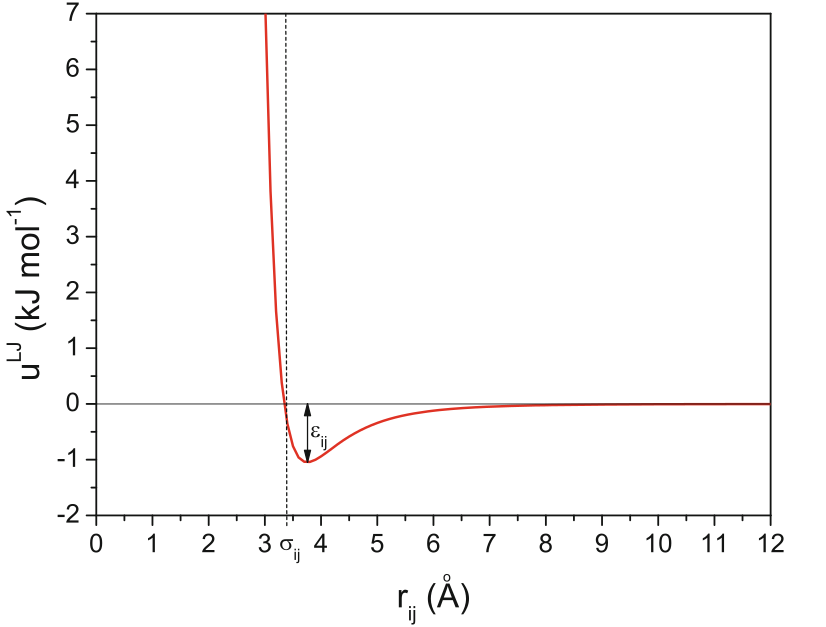
\includegraphics[width=0.8\linewidth]{Figures/lj2}
	\caption{Lennard-Jones potential representation for $\sigma = 1$ and $\epsilon = 1$. }
	\label{fig:lj}
\end{figure}

The potential in Figure \ref{fig:lj} tends to zero and becomes negligible after a specific value of r. Hence, we need to set a cutoff radius in which the potential energy is considered to be zero after it. The point in which the cutoff is defined is generally the one in which the radial distribution function [$g(r)$] is approximately constant. Also, only interactions with the nearest periodic image of the cell are considered for short-range interactions as explained in the Section \ref{icbc}. With this conditions, the calculations of forces and velocities are computationally feasible. The final potential energy function defined by the force field is then expressed by summing all the interactions above:

\begin{equation}
\begin{aligned}
U(r^N) = u_{bs}(d) + u_{ab}(\theta) + u_{bt}(\omega) + u_{q}(r_{ij}) + u_{LJ}(r_{ij}) .
\end{aligned}
\end{equation}
%\subsection{title}
%It is possible to impose movements restrictions on the molecule or even consider the molecule as a rigid body in order to increase the integration step or to follow the modeling of the molecules. Methods for this include the SHAKE, RATTLE and Kamberaj algorithms \cite{RYCKAERT1977327,anderson1983,kamberaj}.

\section{SAFT-$\gamma$ Mie Force Field}


\subsection{SAFT-VR Mie Equation of State (EoS)}

The SAFT-VR Mie equation of state \cite{lafitte2013} is the basis for the SAFT-$\gamma$ Mie coarse-grained force field \cite{avendano2011}, which was the force field used to model the molecules used in the simulations carried out in this dissertation. This EoS was initially developed by \citeonline{lafitte2013} to describe chain molecules formed from fused segments interacting via the Mie attractive and repulsive potential. The Mie potential is a type of generalized Lennard-Jones potential that can be used to explicitly describe repulsive interactions of different hardness/softness and attractive interactions of different ranges, and is given by
\begin{equation}
U_{Mie}(r) = \epsilon\frac{\lambda_r}{\lambda_r - \lambda_a} \left(\frac{\lambda_r}{\lambda_a} \right)^{\left( \frac{\lambda_a}{\lambda_r - \lambda_a} \right)}
\left[ \left(\frac{\sigma}{r} \right)^{\lambda_r} - \left(\frac{\sigma}{r} \right)^{\lambda_a} \right],
\label{eqn:miepotential}
\end{equation}
where $\lambda_r$ is the repulsive exponent and $\lambda_a$ is the attractive exponent. The SAFT-VR Mie equation uses the \citeonline{bh1976} high perturbation expansion of the Helmholtz free energy up to the third order and an improved expression for the  radial distribution function (RDF) of Mie monomers at contact to obtain an equation able to give an accurate theoretical description of the vapor-liquid equilibrium and second derivative properties \cite{lafitte2013}. For a non-associating fluid, the Helmholtz free energy is
\begin{equation}
\frac{A}{N\kappa_{b}T} = a = a^{IDEAL} + a^{MONO} + a^{CHAIN}, 
\label{eqn:miehelm}
\end{equation}
or, depending on the molecule type, the free energy can be equal to
\begin{equation}
\frac{A}{N\kappa_{b}T} = a = a^{IDEAL} + a^{MONO} + a^{RING}.
\label{eqn:miehelmring}
\end{equation}

Here, $a^{IDEAL}$ is the ideal contribution for a mixture. It is given by
\begin{equation}
a^{IDEAL} = \sum_{i=1}^{N_{c}} x_{i}\ln{(\rho_{i}{\Lambda_{i}}^3)} -1 ,
\label{eqn:aideal}
\end{equation}
where $x_{i}=N_{i}/N$ is the molar fraction of component i, $N_{i}$ is the number of molecules of each component, $\rho_{i}=N_{i}/V$ is the number density, and $\Lambda_{i}^3$ is the de Broglie thermal wavelength. Also in Eq. \ref{eqn:miehelm}, $a^{MONO}$ is the monomer contribution, which  describes interactions between Mie segments and can be expressed, for a mixture, as
\begin{equation}
a^{MONO} = \left(\sum_{i=1}^{N_{c}} x_{i}m_{s,i} \right)a^{M} .
\label{eqn:amonomer}
\end{equation}

In the equation above, $m_{s,i}$ is the number of spherical segments making up the molecule i and $a^{M}$  is the monomer dimensionless Helmholtz free energy. $a^{M}$ is expressed as a third-order perturbation expansion in the inverse temperature \cite{bh1976}:
\begin{equation}
a^{M} = a^{HS}+\beta{a_{1}}+\beta{a_{2}}^2+\beta{a_{3}}^3 . 
\label{eqn:aM}
\end{equation}

Here, $a^{HS}$ is the hard-sphere dimensionless Helmholtz free energy for a mixture and is given by:
\begin{equation}
a^{HS} = \frac{6}{\pi\rho_{s}}\left[\left(\frac{\zeta^3_2}{\zeta^2_3}-\zeta_0 \right)\ln(1-\zeta_3)+\frac{3\zeta_{1}\zeta_{2}}{1-\zeta_3}+ \frac{\zeta^3_2}{\zeta_{3}(1-\zeta_3)^2}\right] .
\label{eqn:hs}
\end{equation}

The variable $\rho_{s}=\rho\sum_{i}^{N_c} x_{i}m_{s,i}$ is the total number density of spherical segments and $\zeta_l$ are the moments of the number density:
\begin{equation}
\zeta_l = \frac{\pi\rho_s}{6}\left(\sum_{i=1}^{N_c} x_{s,i}d_{ii} \right), \quad l = 0,1,2,3 ,
\label{eqn:zetal}
\end{equation}
where $x_{s,i}$ is the mole fraction of segments. It is related to the mole fractions of all component ($x_i$) by:
\begin{equation}
x_{s,i} = \frac{m_{s,i}x_i}{\sum_{k=1}^{N_c} m_{s,k}x_{k} } .
\label{eqn:xsi}
\end{equation}


The effective hard-sphere diameter $d_{ii}$ for the segments is
\begin{equation}
d_{ii} =\int_{0}^{\sigma_{ii}} \left \lbrace 1 - \exp \left [-\beta U^{Mie}_{ii}(r) \right ] \right \rbrace dr .
\label{eqn:diameter}
\end{equation}


The integral in Eq. \eqref{eqn:diameter} is normally obtained by means of a 5-point Gauss-Legendre quadrature \cite{papa2014}. For brevity, the detailing of the other terms of Eq. \eqref{eqn:aM} are available at the Appendix \ref{restodaseq}. The term $a^{CHAIN}$ in Eq. \ref{eqn:miehelm} corresponds to the chain contribution. This chain formation of $m_{s}$ tangentially bonded Mie segments is based on the first-order perturbation theory (TPT1)  \cite{papa2014} and can be expressed as
\begin{equation}
a^{CHAIN} =-\sum_{i=1}^{N_{c}} x_{i}(m_{s,i} - 1)\ln \left [ g_{ii}^{Mie}(\sigma_{ii}) \right] .
\label{eqn:achain}
\end{equation}

The term $g_{ij}^{Mie}(\sigma_{ij})$ correspond to the radial distribution function (RDF) of the hypothetical Mie system evaluated at the effective diameter. It is obtained with the following perturbation expansion
\begin{equation}
\begin{aligned}
g_{ij}^{Mie}(\sigma_{ij}) =g_{d,ij}^{HS}(\sigma_{ij})\exp \left [\beta\epsilon \frac{g_{1,ij}(\sigma_{ij})}{g_{d,ij}^{HS}(\sigma_{ij})} + (\beta\epsilon)^{2} \frac{g_{2,ij}(\sigma_{ij})}{g_{d,ij}^{HS}(\sigma_{ij})} \right] .
\end{aligned}
\label{eqn:gmie}
\end{equation}


In the equation above, $g_{d,ij}^{HS}$ is equal to 

\begin{equation}
\begin{aligned}
g_{d,ij}^{HS}(\sigma_{ij}) = \exp (k_{0} + k_{1} x_{0,ij} + k_{2} x_{0,ij}^{2} + k_{3} x_{0,ij}^{3}) ,
\end{aligned}
\label{eqn:ghs}
\end{equation}
where $x_{0,ij} = \sigma_{ij}/d_{ij}$ and $k_{1}, k_{2},$ and $k_{3}$ are density dependent coefficients. These coefficients and the other terms of Eq. \ref{eqn:gmie} are available at Appendix \ref{restodaseq}.  

The ring contribution ($a^{RING}$) in Eq. \ref{eqn:miehelmring} have two forms for rings formed from tangentially bonded segments. The first was developed by \citeonline{lafitte2012}. It considers that the difference between a chain and a ring molecule is that the latter has one more bond that is connecting the first segment to the last. With this assumption, Eq.~\eqref{eqn:achain} can be adapted to rings by
\begin{equation}
a^{RING} =-\sum_{i=1}^{N_{c}} x_{i}m_{s,i}\ln[g_{ii}^{Mie}(\sigma_{ii})] .
\label{eqn:aringlafitte}
\end{equation}

According to \citeonline{lafitte2012}, Eq. \eqref{eqn:aringlafitte} needs an additional parameterization with molecular simulation data so that the EoS can  be used in molecular simulations, but this additional parameterization is not necessary when we are modeling chain molecules. Recently, \citeonline{muller2017} tried to correct this inconsistency. They developed a Helmholtz free energy equation for rings based on the work of \citeonline{muller1993}, who obtained rigorous expressions for hard-sphere fluids with molecular geometries of rings with $m_s=3$. The final expression developed for the dimensionless Helmholtz free energy due to ring formation is
\begin{equation}
a^{RING} =-\sum_{i=1}^{N_{c}} x_{i}\left (m_{s,i}-1+\chi_{i}\eta_{i} \right )\ln \left [g_{ii}^{Mie}(\sigma_{ii}) \right] ,
\label{eqn:aringmuller}
\end{equation}
where $\eta_{i}=m_{s,i}\rho_{i}\sigma_{ii}^{3}/6$ is the packing fraction of the atom i and $\chi_{i}$ is a parameter which depends on $m_{s,i}$ and on the geometry of the ring of each component i. For a value of $\chi=0$, Eq. \eqref{eqn:aringmuller} is equal to Eq. \eqref{eqn:achain}. In addition, the equation corresponds to a system of hard sphere triangles when $\chi=1.3827$. \citeonline{muller2017} also calculated values of $\chi$ for $m_{s}=3,m_{s}=4,m_{s}=5$, and $m_{s}=7$ with pseudo-experimental data from molecular dynamics (MD) for a defined pure fluid with $\epsilon/\kappa_{b} = 250 K$, $\sigma = 3.0 \dot{A}$, $\lambda_{r} = 11$, and $\lambda_{r} = 6$. Values of $\chi$  for some of the geometry estimated in their article can be seen in \figref{ringqsi}.
\begin{figure}[th]
	\centering
	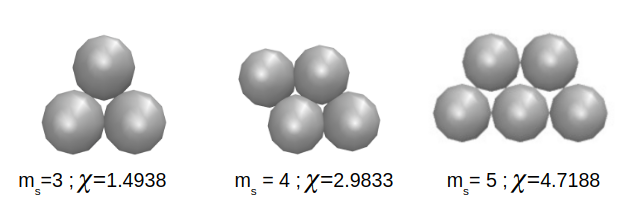
\includegraphics[scale=0.5]{Figures/mullergeo.png}
	\caption{Values for parameter $\chi$ according to the ring geometry. Adapted from \citeonline{muller2017}.}
	\label{ringqsi}
\end{figure}

\citeonline{lafitte2013} also suggested mixing rules for this EoS parameters based on Lorentz-Berthelot combining rules \cite{rowlinson}:
\begin{equation}
\sigma_{ij} =\frac{\sigma_{ii}+\sigma_{jj}}{2},
\label{eqn:sigmamix}
\end{equation}
\begin{equation}
d_{ij} =\frac{d_{ii}+d_{jj}}{2},
\label{eqn:dmix}
\end{equation}
\begin{equation}
\lambda_{k,ij} -3 =\sqrt{(\lambda_{k,ii}-3)(\lambda_{k,jj}-3)},  \quad k=r,a,
\label{eqn:lambdamix}
\end{equation}
\begin{equation}
\epsilon_{ij} =(1-k_{ij})\frac{\sqrt{\sigma_{ii}^{3}\sigma_{jj}^{3}}}{\sigma_{ij}^{3}}\sqrt{\epsilon_{ii}\epsilon_{jj}}.
\label{eqn:epsmix}
\end{equation}

The $k_{ij}$ is a binary interaction parameter to correct the deviations of the mixing rule for chemically distinct compounds that can be fitted to experimental or molecular simulation data. This necessity of an additional parameter raises the question of the quality of these mixing rules and make us wonder if new mixing rules could be used to describe the mixing potential well parameter. Since these were the available mixing rules and the ones employed by other papers that used this force field, we ended up using Eqs. \ref{eqn:sigmamix} to \ref{eqn:epsmix} in our study. However, the binary interaction parameter was only necessary for aqueous mixtures in our study.  


\subsection{Parameter Estimation for the SAFT-$\gamma$ Mie Force Field}\label{parsaft}

The SAFT-$\gamma$ Mie Force Field uses a top-down coarse-graining methodology in its parameterization. This methodology aims to obtain the intermolecular parameters from macroscopic experimental data such as fluid-phase equilibrium or interfacial tension data. The idea is that the force field parameters estimated with the SAFT-VR Mie EoS can be used in molecular simulations since both the equation of state and the force field use the same explicit intermolecular potential model (Mie potential). This correspondence between models has been used to parametrize a variety of fluids \cite{ervik2016}. This force field has the advantage of incorporating the degrees of freedom provided by the use of the Mie Potential \cite{herdes2015}. This flexibility offers the exploration of a vast parameter space without using an iterative simulation scheme \cite{avendano2011}. Despite these advantages, the force field can be restricted by the shortcomings of the equation of state. As an example, the lack of an association term in the equation can cause an inadequate representation of the properties of hydrogen bonding compounds.

Each substance has initially five parameters to be estimated ($m_s,\ \sigma,\ \epsilon,\ \lambda_{r},$ and $, \lambda_{a}$) according to Eq. \eqref{eqn:miepotential}. The number of segments is usually fixed in an integer value since each segment represents one pseudo atom. The attractive parameter is generally  fixed due to its  high correlation with the repulsive parameter. Usually, the chosen value for this parameter is 6, corresponding to the London model, which is a good representation of the dispersion scale of most simple fluids that do not have strong polar interactions \cite{ramrattan2015,herdes2015}. There are two strategies to obtain the parameters: one is by fitting the SAFT-VR Mie EoS to experimental data such as vapor pressure, liquid density and the other one is by using corresponding states parametrization. The first was the one followed in this dissertation. Generally, this approach minimizes the following unweighted least-squares objective function:

\begin{equation}
\begin{aligned}
\min\limits_{\sigma,\epsilon,\lambda_{r}} F_{obj}= \sum_{i=1}^{N_{p}} \left[\frac{P_{v}^{SAFT}(T_{i},\sigma,\epsilon,\lambda_{r})-P_{v}^{exp}(T_{i})}{P_{v}^{exp}(T_{i})} \right]^2 +\\
\sum_{i=1}^{N_{p}} \left[\frac{\rho_{l}^{SAFT}(T_{i},\sigma,\epsilon,\lambda_{r})-\rho_{l}^{exp}(T_{i})}{\rho_{l}^{exp}(T_{i})} \right]^2 ,
\end{aligned}
\label{eqn:fobj}
\end{equation}
where $N_{p}$ is the number of experimental points, $P_{v}$ is the vapor pressure, and $\rho_{l}$ is the saturated liquid density. Other properties that can be used in the estimation are interfacial tension and speed of sound, for instance. The multiple parameters of the model make it necessary the use of a wide range of experimental data since multiple solutions may be found for the fit. Therefore, one needs to be careful in deciding the level of coarse-graining (i.e. the choice of parameter $m_{s}$) and the subsequent parameter space so as to avoid some physical inconsistencies such as a premature freezing \cite{lobanova2015}.

\citeonline{lafitte2012} suggested that two correction factors ($c_{\sigma}$ and $c_{\epsilon}$) should be estimated with simulation data when using Eq. \eqref{eqn:aringlafitte} for the ring contribution. They are related to the EoS parameters by scaled parameters:

\begin{equation}
\sigma^{scaled} = c_{\sigma}\sigma^{SAFT}.
\label{eqn:csigma}
\end{equation}
\begin{equation}
\epsilon^{scaled} = c_{\epsilon}\epsilon^{SAFT}.
\label{eqn:ceps}
\end{equation}

According to \citeonline{lafitte2012}, these corrections are necessary because the approximations employed in the EoS theory generate discrepancies between molecular simulations and the EoS for ring molecules modeled with Eq. \eqref{eqn:aringlafitte}. However, this new parameterization is not necessary when using Eq. \eqref{eqn:aringmuller} as the ring contribution or when we are modeling chain molecules with Eq. \ref{eqn:achain}. This fact makes the strategy of \citeonline{lafitte2012} inconsistent since parameterization with molecular simulation should not be necessary according to the overall idea of this force field. Furthermore, the use of molecular simulation data highly increases the time spent on the parameterization process. The objective function for the estimation of the correction parameter is given by

\begin{equation}
\begin{split}
\min\limits_{c_{\sigma},c_{\epsilon}} F_{obj}= \sum_{i=1}^{N_{p}} \left[\frac{P_{v}^{sim}(T_{i},\sigma^{SAFT},\epsilon^{SAFT})-P_{v}^{SAFT}(T_{i},\sigma^{scaled},\epsilon^{scaled})}{P_{v}^{sim}(T_{i},\sigma^{SAFT},\epsilon^{SAFT})} \right]^2 + \\
\sum_{i=1}^{N_{p}} \left[\frac{\rho_{liq}^{sim}(T_{i},\sigma^{SAFT},\epsilon^{SAFT})-\rho_{liq}^{SAFT}(T_{i},\sigma^{scaled},\epsilon^{scaled})}{\rho_{liq}^{sim}(T_{i},\sigma^{SAFT},\epsilon^{SAFT})} \right]^2 .
\end{split}
\label{eqn:fobjla}
\end{equation}

The repulsive parameter is maintained in the value found on the minimization of Eq. \eqref{eqn:fobj}. The refined values for $\sigma$ and $\epsilon$ are

\begin{equation}
\sigma^{sim} = \sigma^{SAFT}/c_{\sigma},
\label{eqn:simsigma}
\end{equation}

\begin{equation}
\epsilon^{sim} = \epsilon^{SAFT}/c_{\epsilon},
\label{eqn:simeps}
\end{equation}

The other method to obtain the force field parameters is the corresponding states parametrization \cite{mejia2014}. This method considers that the unweighted volume average of the attractive contribution to the Mie intermolecular potential, $ \, a_{1}$, is the following mean-field approximation

\begin{equation}
a_{1} = 2\pi\rho\sigma^{3}\epsilon\alpha .
\label{eqn:a1corres}
\end{equation}

The van der Waals constant, $\alpha$, considering $ \lambda_{a} = 6$ is related by the Mie exponents by

\begin{equation}
\alpha = \frac{1}{\epsilon\sigma^{3    }} \int_{\sigma}^{\infty} \phi(r)r^{2}dr = \frac{\lambda_{r}}{3(\lambda_{r}-3)}\left(\frac{\lambda_r}{6}\right)^{6/(\lambda_{r} - 6)}  .
\label{eqn:alpha}
\end{equation}

The parameterization in this method starts by using the experimental acentric factor, $\omega$, for each molecule with a fixed value of $ m_{s}$ to obtain the value of the repulsive exponent with the following Padé series:

\begin{equation}
\lambda_{r} = \frac{\sum_{i=0} a_{i}\omega^{i}}{1+\sum_{i=1} b_{i}\omega^{i}} ,  
\label{eqn:lambdaco}
\end{equation}
where $a_{i}$ and $b_{i}$ are parameters that are dependent on the number of segments. A table with these parameters is presented in the original paper \cite{mejia2014}. The van der Waals constant can be found by substituting $\lambda_{r}$ into Eq. \eqref{eqn:alpha}. The reduced critical temperature $T_{c}^{*}$ is related to $\alpha$ by a Padé series: 

\begin{equation}
T_{c}^{*} = \frac{\sum_{i=0} c_{i}\alpha^{i}}{1+\sum_{i=1} d_{i}\alpha^{i}}   .
\label{eqn:tc}
\end{equation}

The values of $c_{i}$ and $d_{i}$ are also available in the original paper. The reduced temperature of the equation above is used in conjunction with the experimental critical temperature, $ T_{c}$, to find the energy parameter with the relation below:

\begin{equation}
T_{c}^{*} = \frac{\kappa_{b}T_{c}}{\epsilon}   .
\label{eqn:epscorre}
\end{equation}

The diameter parameter, however, is not obtained with the critical properties, but with the reduced liquid density at the reduced temperature of $0.7$ ($\rho_{T_{r}=0.7}$). This density is also obtained with a Padé series using parameters by \citeonline{mejia2014}:

\begin{equation}
\rho_{T_{r}=0.7}^{*} = \frac{\sum_{i=0} j_{i}\alpha^{i}}{1+\sum_{i=1} k_{i}\alpha^{i}} .
\label{eqn:denscorre}
\end{equation}

The relation between the equation above, $\sigma$ and the experimental density is given by

\begin{equation}
\rho_{T_{r}=0.7}^{*} = \rho_{T_{r}=0.7}\sigma^{3}N_{av},   
\label{eqn:sigmacorre}
\end{equation}
where $N_{av}$ is the Avogadro number. This corresponding states method has the advantage of only requiring critical data, which is available for a great range of fluids, and liquid density data. The parameters found with this strategy are available at an online database \cite{ervik2016}.     

The binary interaction parameter $k_{ij}$ of Eq. \eqref{eqn:epsmix} is necessary to adjust the mixture behavior of chemically distinct components. Normally, it is estimated by minimizing the difference between experimental binary vapor-liquid equilibrium or interfacial tension data and the SAFT-VR Mie EoS output data \cite{muller2017,lobanova2016}. The objective function is similar to: 

\begin{equation}
\begin{aligned}
\min\limits_{k_{ij}} F_{obj}= \sum_{k=1}^{N_{p}} \left(\frac{P_{v}^{SAFT}(T_{k},x,k_{ij})-P_{v}^{exp}(T_{k},x)}{P_{v}^{exp}(T_{k},x)} \right)^2 +\\
\sum_{k=1}^{N_{p}} \left(\frac{\rho_{l}^{SAFT}(T_{k},x,k_{ij})-\rho_{l}^{exp}(T_{i})}{\rho_{l}^{exp}(T_{i})} \right)^2 .
\end{aligned}
\label{eqn:fobjmix}
\end{equation}

However, \citeonline{ervik20162} used molecular simulation results to fit the parameter to the interfacial tension data. The strategy they followed was to carry out simulations in three values of $k_{ij}$ first and, after, refine the parameter until a value in good agreement with the experimental data is found. We decided to follow this strategy in our estimations of $k_{ij}$ since the estimation with the EoS did not provide satisfactory results for the hydration free energy calculations.  

\section{Solvation Free Energy Calculations Based on Molecular Dynamics}
% background topics

Using the SAFT-$\gamma$ Mie Force Field described in the section above, we carried out solvation free energy molecular dynamics simulations. The free energies we are trying to calculate can be expressed as averages over ensembles of atomic configurations generated using Monte Carlo or Molecular Dynamics techniques. In the canonical ensemble, the free energy is given by  

\begin{equation}
\label{eq:fcano}
\begin{aligned}
F(N,V,T) = -\kappa_{b}T \ln Q(N,V,T).
\end{aligned}
\end{equation}

Recall that $Q(N,V,T)$ is the partition function of the canonical ensemble, expressed as

\begin{equation}
\label{eq:partican}
\begin{aligned}
Q(N,V,T) =\frac{\epsilon_{0}}{h^{3N}N!} \int d^{n}p d^{n}r \exp \left[ -\beta \left( \sum_{i=1}^{N}\dfrac{p_{i}^{2}}{2m_{i}} + U(r_{1},..,r_{n}) \right)
\right] .
\end{aligned}
\end{equation}

The Gibbs free energy, the object of study in this dissertation, is given by

\begin{equation}
\begin{aligned}
G(N,P,T) = -\kappa_{b}T ln \Delta (N,P,T),
\end{aligned}
\end{equation}
where $\Delta (N,P,T)$ is the partition function of the isothermal-isobaric ensemble:

\begin{equation}
\begin{aligned}
\Delta (N,P,T) = \frac{1}{V_{0}} \int_{0}^{\infty} dV \int d^{n}p d^{n}r \exp \left[ -\beta \left( \sum_{i=1}^{N}\dfrac{p_{i}^{2}}{2m_{i}} + U(r_{1},..,r_{n}) + PV(r_{1},..,r_{n}) \right) \right].
\end{aligned}
\end{equation}

Evaluating the partition function is an often unfeasible task, but we are interested in calculating only the Gibbs free energy difference between two states of a system, which is  

\begin{equation}
\begin{aligned}
\Delta G_{AB} = G_{B} - G_{A}= -\kappa_{b}T ln \left( \frac{\Delta_{B}}{\Delta_{A}}\right) .
\end{aligned}
\end{equation}

Since the masses of particles in states A and B of a system are the same and the Hamiltonian is separable in $K(p)$ and $U(r)$, the moment integrals in the ratio ${\Delta_{B}}/{\Delta_{A}}$ can be simplified into the ratio of the configuration integrals:

\begin{equation}
\label{eq:partiso}
\begin{aligned}
\dfrac{Z_{B}}{Z_{A}} = \dfrac{\int_{0}^{\infty} dV \int d^{n}r \exp \left\lbrace -\beta \left[U(r_{1},..,r_{n}) + PV(r_{1},..,r_{n}) \right]_{B} \right\rbrace}{\int_{0}^{\infty} dV \int d^{n}r \exp \left\lbrace  -\beta \left[U(r_{1},..,r_{n}) + PV(r_{1},..,r_{n}) \right]_{A} \right\rbrace }.
\end{aligned}
\end{equation}

This identity results in the following equation for the Gibbs free energy difference, which does not  require the calculation of the partition function at each state:

\begin{equation}
\label{eq:dif}
\begin{aligned}
\Delta G_{AB} = G_{B} - G_{A}= -\kappa_{b}T ln \left( \frac{Z_{B}}{Z_{A}}\right).
\end{aligned}
\end{equation}

In the case of a study concerning the solvation of a single molecule, the Gibbs free energy difference between end states $A$ and $B$ are, more specifically, the difference between the solute alone in the gas phase and the solute interacting with the solvent. In order to have accurate results for free energy differences, the states need to have sufficient overlap  \cite{klimovich}. The overlap can be achieved by calculating the free energy difference among a series of intermediates states. The result of these differences is independent of the path chosen since free energy is a state function. That is why alchemical states (without physical sense) can be used to link physical states of interest. The solvation free energy calculations are then done through a thermodynamic path in which the solute molecule is gradually inserted into the solvent as illustrated in \figref{thermcy}. According to this path, the free energy of solvation is expressed as

\begin{equation}
\label{eq:freesolv}
\begin{aligned}
\Delta G_{solv} = \Delta G_{1 \rightarrow 4} = \Delta G_{1 \rightarrow 2} + \Delta G_{2 \rightarrow 3} + \Delta G_{3 \rightarrow 4}  - \kappa_{b}T \ln \dfrac{V^{*}}{V^{1}} .
\end{aligned}
\end{equation}

\begin{figure}[th]
	\centering
	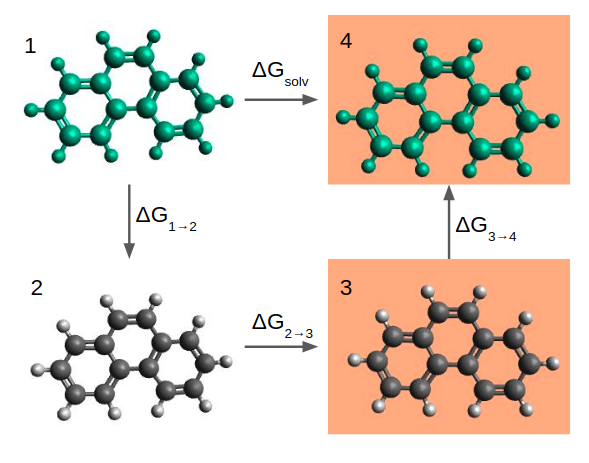
\includegraphics[scale=0.6]{Figures/cicclotermo}
	\caption{Thermodynamic path for computing solvation free energy of a single solute molecule with molecular dynamics. Adapted from \citeonline{klimovich}.}
	\label{thermcy}
\end{figure}

The last term in Eq. \ref{eq:freesolv} accounts for the difference between the mean volume of the simulation box with the solute inserted ($V_{1}$) and the mean volume of the simulation box with only solvent molecules in it ($V^{*}$). However, \citeonline{shirts2013} have shown that this term is negligible with respect to the statistical uncertainty of calculating $\Delta G$. In addition, when we have other solute molecules that are equal to the solute molecule being inserted in the box, another term in Eq. \ref{eq:freesolv} can appear in order to distinguish these molecules \cite{shirts2013}. The  term $\Delta G_{1 \rightarrow 2}$, also represented in \figref{thermcy},  is the solvation free energy associated with turning off the non bonded interactions of the molecule in the gas phase. In the next transformation, $\Delta G_{2 \rightarrow 3}$ is the free energy of moving the non-interacting molecule from the gas phase to the solvent and is equal to zero since the transformation of a non-interacting molecule does not depend on the environment. Lastly, $\Delta G_{3 \rightarrow 4}$ is the free energy required for the non-interaction molecule in the aqueous phase to regain its non-bonded interactions with the solvent.  The solvation free energy calculation can be classified according to the types of non-bonded interactions that are turned off/on in the $1 \rightarrow 2$ and $ 3 \rightarrow 4$ parts of the path. If both non-bonded interactions with the environment and internal interactions are turned off, this is an annihilation free energy calculation. On the other hand, if only non-bonded interactions with the environment are turned off, this is a decoupling free energy calculation \cite{klimovich}. In the latter case, $\Delta G_{1 \rightarrow 2} = 0$ and the $\Delta G_{solv} = \Delta G_{3 \rightarrow 4} $.  

The methods used to carry out the transformations of Figure \ref{thermcy} during the simulation scale the solute charges to zero and then turn off the interactions corresponding to the Lennard-Jones or Mie potential. In order to carry out the latter process, a modified potential with a coupling parameter ($\lambda$) is used. Each $\lambda$ represents an alchemical state. When $\lambda=0$, there is no interaction with the solvent and, when $\lambda=1$, interactions are fully activated. The coupling of the $\lambda$ parameter could be linear, but it could generate numerical problems related to the exponential part of the potential \cite{shirts2013}. We can see in Figure \ref{fig:linearpoten} that a linear coupling of the parameter would cause an abrupt change in the potential energy when the $\lambda$ reaches zero. That is the reason the non-linear softcore scheme \cite{beutler1994} is used to couple the $\lambda$. This scheme makes the potential behave more smoothly in relation to the change of $\lambda$, as can be seen in \figref{fig:SC}. The softcore potential is  

\begin{equation}
\label{eq:softcoreLJ}
\begin{aligned}
U_{LJ}^{sc}(r) {}=& 4\lambda\epsilon \left\lbrace\frac{1}{\left[\alpha(1-\lambda)+ (r/\sigma)^{6}\right]^{2}} - \frac{1}{\alpha(1-\lambda)+(r/\sigma)^{6}}\right\rbrace ,
\end{aligned}
\end{equation}
where $\alpha$ is a constant whose value is  normally assumed to be 0.5.    Based on Eq. \ref{eq:softcoreLJ}, we propose a generalized softcore Mie potential for any value of $\lambda _{r}$ and $\lambda _{a}$. It is given by:

\begin{equation}
\label{eq:softcore}
\begin{aligned}
U^{sc}(r) {}=& \lambda\epsilon\dfrac{\lambda_r}{\lambda_r - \lambda_a} \left(\frac{\lambda_r}{\lambda_a} \right)^{\left( \frac{\lambda_a}{\lambda_r - \lambda_a} \right)} \left\lbrace\dfrac{1}{\left[\alpha(1-\lambda)+ (r/\sigma)^{\lambda_a}\right]^{\lambda_{r}/\lambda_{a}}} - \dfrac{1}{\alpha(1-\lambda)+(r/\sigma)^{\lambda_a}}\right\rbrace .
\end{aligned}
\end{equation}

\begin{figure}[H]
	\centering
	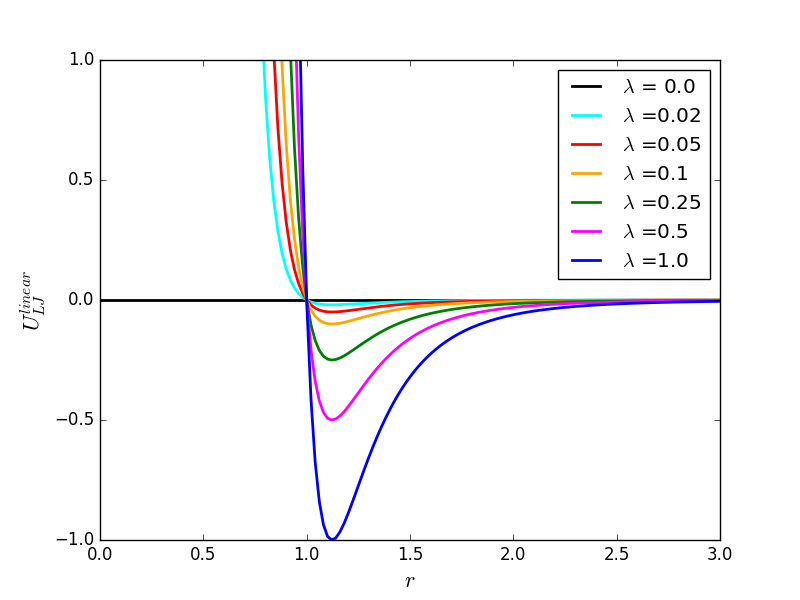
\includegraphics[width=0.8\linewidth]{Figures/linear}
	\caption{Linear coupling of the potential energy, $U^{linear}_{LJ} = \lambda U_{LJ}$, for different values of $\lambda$. Here, $\sigma=1$ and $\epsilon=1$}
	\label{fig:linearpoten}
\end{figure}    

\begin{figure}[H]
	\centering
	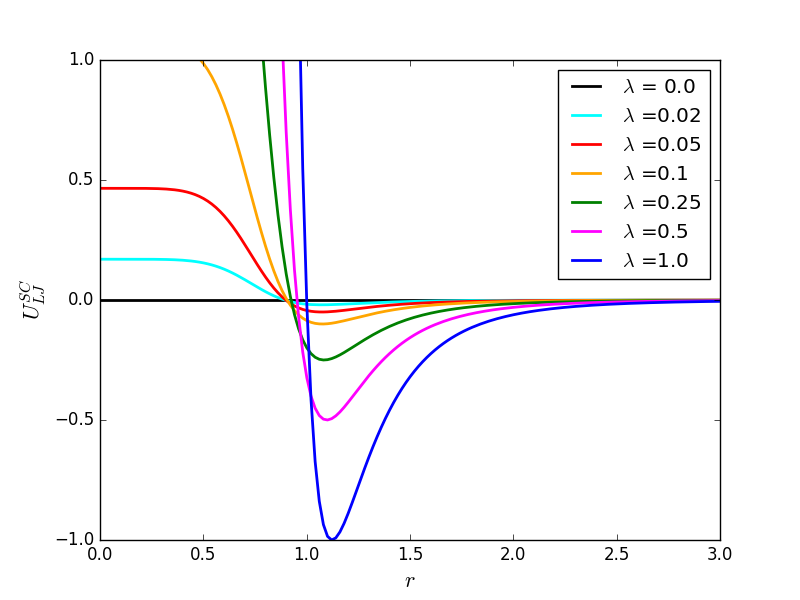
\includegraphics[width=0.8\linewidth]{Figures/soft}
	\caption{Softcore potential, Eq. \ref{eq:softcoreLJ}, for different values of $\lambda$. Here, $\sigma=1$ and $\epsilon=1$.}
	\label{fig:SC}
\end{figure}

Now that we defined our coupled potential, we can then obtain the potential energies related to each alchemical state by doing independent simulations in different values of $\lambda$ or by doing expanded ensemble simulations \cite{lyubartsev}. The latter was the method used in this dissertation, and it is described in Section \ref{ee}. With the potential energies, the next step is to use post-processing methods, such as the MBAR used in this study, to effectively calculate $\Delta G_{3 \rightarrow 4}$.  The solvation free energies can then be used to calculate other properties such as the partition coefficient. This property is a measure of the partitioning of one solute in two solvents (a and b) with different physicochemical characteristics  at a temperature T. It is defined by the following equation when the activity coefficients are assumed to be one \cite{doi:10.1021/ja00036a009}:

\begin{equation}
P = \dfrac{[solute]_{a}}{[solute]_{b}},
\end{equation} 
where $[solute]_{a}$ and $[solute]_{b}$ are the concentration of the solute in the solvent a and b, respectively. Since $P$ is an equilibrium constant, it can be related to free energy change associated with transferring the solute from the phase a to the phase b. Hence, we can define the relation between the partition coefficient and the difference in free energy with the equation bellow \cite{doi:10.1021/ja00036a009}:  

\begin{equation}
\label{eqn:partcoe}
{2.303RT} \log{P}^{a/b} ={\Delta G_{solv}^{a} - \Delta G_{solv}^{b}},
\end{equation}
where 2.303 is a conversion factor.

\section{Expanded Ensemble Method}\label{ee}

We decided to use the Expanded Ensemble method \cite{lyubartsev} in our solvation free energy simulations since it allows a non-Boltzmann sampling scheme of different states in a single simulation. \citeonline{lyubartsev} initially proposed in their paper a sampling scheme of different temperatures, but this idea can be generalized to a sampling scheme of different states or $\lambda 's$ \cite{escobedo2007}. In this scheme, the sampling is done by biasing the phase space exploration process with weights not related to the statistical ensemble. The partition function of the statistical expanded ensemble, $Z^{EE}$, is obtained from the probability distributions corresponding to each $\lambda$. Hence, $Z^{EE}$ is defined as a sum of subensembles $Z_{i}$ in different values of $\lambda$, that is,

\begin{equation}
Z^{EE} = \sum_{i=1}^{N} Z_{i}(\lambda_{i}) exp(\eta_{i}),
\label{eqn:ee}
\end{equation}   
where N is the number of alchemical states, $\eta_{i}$ is the arbitrary weight of the subensemble at each state, and $Z_{i}$ is the configurational partition function of state i. For the isothermal-isobaric ensemble, $Z_{i}$ is given by

\begin{equation}
Z_{i} = \frac{1}{V_{0}} {\int_{0}^{\infty} dV \int d^{n}r^{n} \exp \left \lbrace -\beta_{i} \left[ U(\lambda, r_{1},..,r_{n}) + P_{i}V(r_{1},..,r_{n}) \right] \right \rbrace}.
\end{equation} 

In solvation free energy calculations with molecular dynamics, $\lambda$ corresponds to the coupling parameter of the softcore potential (Eq. \ref{eq:softcoreLJ}). Since we are carrying out molecular dynamic simulations, the sampling of the expanded ensemble is done by performing an arbitrary number of MD  steps followed by a $\lambda$ transition. \citeonline{chodera2011} proved that this type of sampling of the expanded ensemble is similar to the Gibbs sampling method \cite{geman1984,liu2002}. Following the Gibbs method, the sampling of the configuration space $x$ for one state $\lambda_{k}$ during the MD steps is done by using the conditional distribution:

\begin{equation}
\pi(x|\lambda_{k}) = \dfrac{\exp[-\beta u(x,\lambda_{k})]}{\int dx \exp [- \beta u(x,\lambda_{k})]}.
\label{eqn:rhoee1}
\end{equation} 

The state transition in the MD simulation uses the following conditional distribution:

\begin{equation}
\pi(\lambda_{k}|x) = \dfrac{\exp[-\beta u(x,\lambda_{k}) + \eta_{k}]}{ \sum_{k=1}^{K} \exp [- \beta u(x,\lambda_{k})+ \eta_{k}]},
\label{eqn:rhoee2}
\end{equation} 
where $u(x,\lambda_{k})$ is the reduced potential function for the NPT ensemble. There is a variety of acceptance schemes to do the expanded sampling using Eq. \eqref{eqn:rhoee2}, but \citeonline{chodera2011} suggested that the independence sampling \cite{liu2002} is the best strategy to increase the number of uncorrelated configurations. The implementation they suggested consists of updating the state index from $i$ to $j$ by first generating a uniform random number $R$ on the interval $[0,1)$ and then selecting the smallest new value of $j$ that satisfies  the relation

\begin{equation}
R < \sum_{i=1}^{j} \pi(\lambda_{i}|x) .
\label{eqn:relee2}
\end{equation} 

The sampling strategy above depends on a proper selection of weights in order to guarantee an adequate sampling of the states. If there is not a sufficient number of visits to each state, the expanded ensemble becomes deficient in obtaining input data to estimate free energy differences with the methods exposed in Section \ref{SFECM}. Here, we followed the flat-histogram approach \cite{bernd1992,bernd1993,dayal2004} to calculate the weights. This strategy aims to obtain adequate sampling by ensuring that all the states have an equal number of visits, i.e. the ratio of the probability of sampling state i ($\pi_{i}$) to the probability of sampling state $j$ ($\pi_{j}$) is equal to one. Given that $\pi_{i}$ is equal to:

\begin{equation}
\pi_{i} = \dfrac{Z_{i}(\lambda_{i}) exp(\eta_{i})}{Z^{EE}} ,
\label{eqn:wei1}
\end{equation} 
and using Eqs. \ref{eq:dif} and \ref {eq:partiso}, the following relation can be obtained for $\pi_{i}/\pi_{j}=1$:

\begin{equation}
(\eta_{i} - \eta_{j}) = \beta(G_i-G_j).
\label{eqn:weight}
\end{equation}

Eq. \eqref{eqn:weight} proposes that the choice of the weights is dependent on the free energies that we are attempting to obtain. This equation is then solved iteratively with trial simulations. For the first simulation, the values of $\eta$ are set to zero, and the histogram of the states visited is obtained. With this histogram, it is possible to estimate the free energy differences and, since the weights are related to the free energies by Eq. \eqref{eqn:weight}, the next values of $\eta$ can be calculated. This iteration goes on until a uniform distribution is attained. The weights found are then used in a longer simulation to obtain the final solvation free energies.

The choice of the $\lambda$ set corresponding to overlapping alchemical states are crucial to acquire accurate solvation free energies. In this work, the method chosen to obtain the optimal staging of the $\lambda$ domain is the one developed by \citeonline{escobedo2007} with a basis in the study of  \citeonline{1742-5468-2006-03-P03018}. This method targets "bottlenecks" in the simulation. It does that by optimizing $\lambda$ through the minimization of the number of round trips per CPU time between the lowest ($0$) and highest ($1$) values of $\lambda$. This is specifically done by maximizing the steady-state flow $\phi$ of the simulation, which "walks" among the values of $\lambda$. This flow is estimated from a Fick's diffusion type of law:

\begin{equation}
\phi = D(\Lambda) \Pi (\Lambda) \dfrac{dx(\Lambda)}{d \Lambda}.
\label{eqn:stream}
\end{equation}

In the equation above, $\Lambda$ is the actual continuous value of the coupling parameter. This continuous function of $\lambda 's$ is obtained by interpolating the $\lambda$ set linearly. $D(\Lambda)$ is the diffusivity at  state $\Lambda$ and $x(\Lambda)$ is the fraction of times that the trial simulation at state $\Lambda_{i}$ has most recently visited the state $\lambda=1$ as opposed to state $\lambda=0$. The derivative ${dx(\Lambda)}/{d \Lambda}$ is approximated with the central finite differences method. Finally, $\Pi (\Lambda)$ is the probability of visiting $\Lambda$:

\begin{equation}
\Pi (\Lambda) = \dfrac{C^{'} \bar{\Pi} (\lambda)}{\Lambda_{i+1} - \Lambda_{i}}.
\label{eqn:plambda}
\end{equation}

The $C^{'} $ term in the equation above represents a constant and $\bar{\Pi} (\lambda)$ is the arithmetic average of the frequency of visits to the $\Lambda$ state:

\begin{equation}
\bar{\Pi}_{i} (\lambda) = \dfrac{\pi_{i+1} - \pi_{i}}{2}.
\label{eqn:barplambda}
\end{equation}

The $\phi$ is maximum when the optimal probability $\Pi^{'}(\Lambda_{i})$ of visiting state $\Lambda_{i}$ is proportional to $1/\sqrt{D(\Lambda)}$ \cite{trebst2004}. With that information, it is possible to estimate the diffusivity using one trial simulation with the following equation:

\begin{equation}
\begin{aligned}
D(\Lambda) {}=& \dfrac{\Lambda_{i+1} - \Lambda_{i}}{\bar{\Pi} (\lambda) {dx(\Lambda)}/{d \Lambda}}, \quad \Lambda_{i} < \Lambda < \Lambda_{i+1}.
\end{aligned}
\label{eqn:diff}
\end{equation}    
Hence, we can calculate $\bar{\Pi} $ and, consequently, the cumulative probability, which is used to obtain the new $\lambda$ states by

\begin{equation}
\Phi = \int_{\lambda =0}^{\lambda =1} \Pi^{'}(\Lambda_{i}) d \Lambda = \dfrac{i}{K},
\label{eqn:cumfun}
\end{equation}
where $K$ is the total number of $\lambda$ states. In order to carry out our solvation free energy simulations, we obtained these cumulative probabilities for every $\lambda$ set we estimated. A graphical demonstration of the relation between the optimized coupling parameters and the cumulative probability of Eq. \ref{eqn:cumfun} is presented in Figure \ref{fig:optimized_cdfexeample}.

\begin{figure}[h]
	\centering
	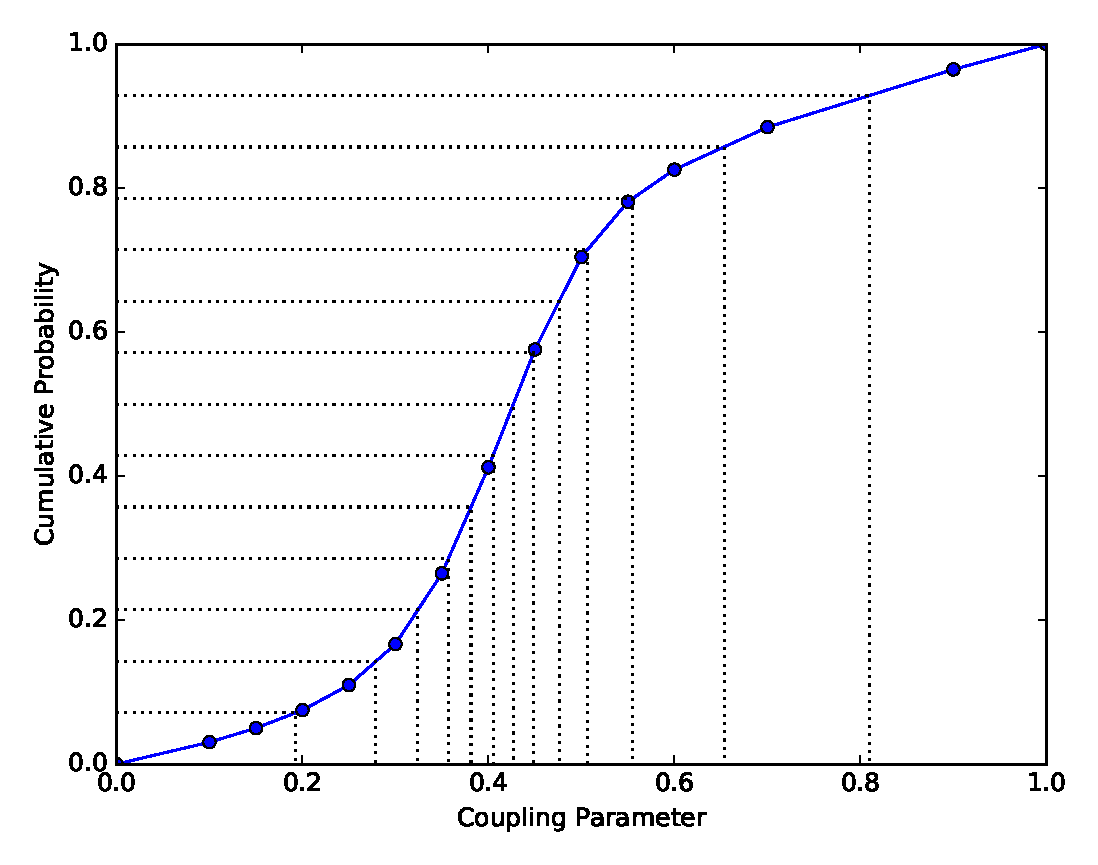
\includegraphics[width=0.8\linewidth]{Figures/optimized_cdfexeample}
	\caption{Relation between the optimized coupling parameters and the cumulative probability used to obtain them.}
	\label{fig:optimized_cdfexeample}
\end{figure}
\FloatBarrier
\section{Multistate Bennett Acceptance Ratio (MBAR)}\label{mbar}

We presented in the sections above the methods used to obtain the total potential energies of each alchemical state with molecular dynamics, and, in this section, we are going to discuss the methodology utilized to estimate the solvation free energies with these data. The MBAR method \cite{mbar} is based on the free energy perturbation. It is a maximum likelihood method which proposes an estimator that computes free energies and their uncertainties of all $K$ states by minimizing the $K \times K$ matrix of variances for a simulation with $N_{j}$ uncorrelated samples in equilibrium. For each of the $\lbrace x_{i,n } \rbrace ^{N_{i}}_{n=1 }$ configurations of i, the following probability distributions are sampled:
\begin{equation}
p_{i}(x) = \frac{q_{i}(x)}{c_{i}},
\end{equation}

\begin{equation}
c_{i} = \int dx q_{i}(x),
\end{equation}
where $q_{i}(x)=\exp[-u_{i}(x)]$ and $u_{i}$ is the reduced potential energy of each state, defined for a an alchemical transformation by $u_{i} (x)= \beta_{i} [U_{i}(x)]$. In addition, $c_{i}$ is a normalization constant.  The free energies are estimated from the ratio of this constant in each state, since

\begin{equation}
\Delta f_{ij} = f_{i} - f_{j} = - \ln \frac{c_{j}}{c_{i}}  = -\ln \frac{\int dx q_{j}(x)}{\int dx q_{i}(x)} .
\label{eqn:mbar1}
\end{equation}

\citeonline{mbar} then proposed the following arbitrary function:

\begin{equation}
c_{i} \langle \alpha _{ij} q_{j} \rangle _{i}  =  c_{j} \langle \alpha _{ij} q_{i} \rangle _{j} .
\end{equation}

Using the equation above for every state  K, the following relation is obtained:

\begin{equation}
\label{eq:mbar1}
\sum_{j=1}^{K} \frac{\hat{c_{i}}}{N_{i}} \sum_{n=1}^{N_{i}} \alpha _{ij} q_{j} (x_{i,n}) =  \sum_{j=1}^{K} \frac{\hat{c_{j}}}{N_{j}} \sum_{n=1}^{N_{j}} \alpha _{ij} q_{i} (x_{j,n}) .
\end{equation}

\citeonline{mbar} suggested the following equation for the arbitrary term $\alpha _{ij}$ in order to minimize the variance:

\begin{equation}
\label{eq:mbar2}
\alpha _{ij} (x) = \frac{N_{j} \hat{c_{i}} ^{-1}}{\sum_{k=1}^{K} N_{k} c_{i} ^{-1} q_{k}(x)} .
\end{equation}

Assuming that the sampling is carried out following Boltzmann statistics, Eqs. \eqref{eq:mbar1} and \eqref{eq:mbar2} can be rearranged to obtain the free energy estimator, which is solved self consistently:  

\begin{equation}
\label{eq:mbar}
\begin{aligned}
f_{i} = \frac{1}{\beta}ln \sum_{k=1}^{K} \sum_{n=1}^{N_{k}}
\dfrac{\exp[-\beta u_{i}(x_{kn})]}{\sum_{l=1}^{K} N_{l} \exp \lbrace \beta [f_{l} - u_{l}(x_{kn})] \rbrace} .
\end{aligned}
\end{equation}

The equation above requires the evaluation of the potential energy  of every  uncorrelated configuration $n$ for all K states [$u_{i}(x_{kn})$] and for all uncorrelated configuration snapshots ($N_{k}$) from state $k$. With the free energies, we compute the free energy differences between states with Eq. \ref{eqn:mbar1}. The statistical variance resulting from free energy estimation is given by the covariance matrix ($s$):

\begin{equation}
\begin{aligned}
\delta _{ij}^{2} s_{ij} = s_{ii}^{2} + s_{jj}^{2} - 2 s_{ij}.
\end{aligned}
\end{equation}

The MBAR method explained here can be considered as a limiting case of the 
Weighted Histogram Analysis Method (WHAM) \cite{wham} for computing free energies. WHAM equations become equal to Eq. \eqref{eq:mbar} if the histogram width tends to zero. Despite this, the MBAR is still more suited than the WHAM because it does not have the bias associated with the discretization and allows the calculation of an error estimate \cite{mbar}.

\section{Gibbs Ensemble Monte Carlo (GEMC)}\label{gemc}

In the initial steps of this research, we estimated the SAFT-$\gamma$ Mie force field parameters of phenanthrene with the methodology proposed by \citeonline{lafitte2012}. This approach required liquid-vapor equilibrium data obtained with molecular simulation, as it is described in Section \ref{parsaft}. Hence, we carried out Monte Carlo simulations at the Gibbs Ensemble \cite{papa1987} since this ensemble is commonly used to study phase coexistence with molecular simulation. In addition to that, this method does not use an explicit interface, which can hinder the determination of bulk phase behavior of small systems with long-range interactions \cite{C1FD00090J}. 

Before talking in more detail about this ensemble, we are going to discourse on Monte Carlo simulations briefly. The Monte Carlo (MC) approach is another method for generating atomic trajectories in order to obtain macroscopic properties. Rather than using the numerical integration of Newton's equations of motion, the trajectories are obtained stochastically in the Monte Carlo approach. The positions are evolved by random moves or perturbations (MC steps) acquired with the Metropolis method \cite{1953JChPh..21.1087M}. Hence, the trajectories are not predictable from the set of initial positions. The Metropolis method is a Markov process, that is, a stochastic process in which the configurations change randomly with time and only depends on the states and their directly preceding states, but not on the previous configurations \cite{raabe}. The random move is constructed in such a way that the probability of visiting a particular point $r^{N}$ is proportional to the Boltzmann factor $exp[-\beta U(r^{N})]$ \cite{frenkel}. The construction of a  particle displacement according to \citeonline{1953JChPh..21.1087M} can be briefly summed up as:

1. Pick a random particle, and calculate its energy $U(r^{N})$.

2. Perturb the particle by randomly displacing  it, $r' = r +\Delta r$. Where $\Delta r$ is a perturbation randomly chosen from a defined interval of maximum displacement ($[- \delta _{max},\delta _{max}]$). Calculate the energy with the new positions $U(r'^{N})$.

3. Accept the move from $r^{N}$ to $r'^{N}$ with the probability:
\begin{equation}
acc_{A \rightarrow B} = min \lbrace 1,exp[-\beta U(r'^{N}) + \beta U(r^{N}) ] \rbrace .
\end{equation}

The values of maximum displacement are defined iteratively in order to obtain acceptance rates of 25-50\% in step 3   \cite{Frenkel2013}. Monte Carlo simulations are interesting when we need to calculate properties in different thermodynamic ensembles, such as the Gibbs Ensemble used in this dissertation. The phase coexistence at this ensemble is obtained with simultaneous Monte Carlo (MC) simulations of two boxes with periodic boundary conditions, representing a two-phase system. The boxes exchange molecules, energy, and volume between them. Equilibrium is obtained through MC steps that consist of translation and rotation moves, volume exchange moves, and random exchanges of molecules between the boxes. For the phase equilibrium of multi-component systems, the GEMC simulations should be carried out at the NPT (constant number of particles, pressure, and temperature) ensemble to obey the requirement of an additional degree of freedom for mixtures. In turn, the simulation of single component systems is carried out at a constant number of particles, temperature, and volume (NVT) since the two-phase region would be a line for this system at constant pressure and temperature \cite{frenkel}. The partition function of the GEMC-NVT ensemble is obtained by considering that the particles in both boxes are subjected to the same intermolecular interactions. Also, volumes and number of particles of the box ($N_{1}$,$\, N_{2}$,$\, V_{1}$ and $V_{2}$) can vary while the total volume ($V$) and the total number of particles ($N$) remain constant ($N = N_{1} + N_{2}$,$\, V = V_{1} + V_{2}$). Therefore, the partition function is

\begin{equation}
\begin{aligned}
Q(NVT) {} \equiv & \sum_{N_{1}}^{N} \dfrac{1}{V \Lambda ^{3N} N_{1}!(N-N_{1})!} \int_{0}^{V} V_{1}^{N_{1}} V_{2}^{N_{2}} dV_{1} \\
& \int  \exp[-\beta U(x_{1}^{N_{1}})] dx_{1}^{N_{1}} \int  \exp[-\beta U(x_{2}^{N_{2}})] dx_{2}^{N_{2}}.
\end{aligned}
\label{eqn:gepart}
\end{equation}

In order to define the acceptance rules for the MC moves and compute any property of interest, it is necessary to know the probability of finding the configuration with $N_{1}$ particles in box 1 with volume $V_{1}$ and positions $x_{1}^{N_{1}}$ and $x_{2}^{N_{2}}$. This probability is given by:

\begin{equation}
\pi(x_{1}^{N_{1}},x_{2}^{N_{2}},N_{1},N_{2},V_{1},V_{2}) \propto \dfrac{V_{1}^{N_{1}}V_{2}^{N_{2}}}{N_{1}!N_{2}!} \exp[-\beta U(x_{1}^{N_{1}}) -\beta U(x_{2}^{N_{2}})] .
\label{eqn:geprob}
\end{equation}

The acceptance criterion for the translation and rotation moves from configuration A    to configuration B is similar to the conventional NVT MC method and is equal to:

\begin{equation}
acc_{A \rightarrow B} = \min \lbrace 1,\exp[-\beta U(x_{A}^{N_{1}}) -\beta U(x_{B}^{N_{1}})] \rbrace .
\label{eqn:drprob}
\end{equation} 

The volume exchange moves take place by exchanging an amount $\Delta V$ between the boxes to achieve pressure equilibrium. $\Delta V$ can be chosen from a uniform distribution based on the maximum variation of volume ($\delta V_{max}$) defined with probability $1/\delta V_{max}$ \cite{frenkel}. The acceptance rule for these moves is: 

\begin{equation}
acc_{A \rightarrow B} = \min \left \lbrace 1, \left(\dfrac{V_{1}^{B}}{V_{1}^{A}} \right)^{N_{1}=1} \left( \dfrac{V_{2}^{B}}{V_{2}^{A}} \right)^{N_{2}+1} \exp[-\beta U(x_{A}^{N}) -\beta U(x_{B}^{N})] \right \rbrace .
\label{vprob}
\end{equation}

Particle exchange moves are carried out to obtain the equality of chemical potential between the boxes. One particle from one box is removed and then added to a random location in the other box. The criteria to accept or reject this type of move is:

\begin{equation}
acc_{A \rightarrow B} = \min \left \lbrace 1, \dfrac{N_{1}V_{2}}{N_{2}V_{1}}  \exp[-\beta U(x_{A}^{N}) -\beta U(x_{B}^{N})] \right \rbrace .
\label{moleprob}
\end{equation}

This method has been widely used to calculate phase equilibrium, but its performance is poor for the region near the critical point due to large density fluctuations. The GEMC method also has poor performance for dense systems since the particle exchange moves have a low acceptance rate \cite{978-94-017-0765-7}.  





